\documentclass[12pt,twoside,a4paper,titlepage]{article}

\usepackage[swedish,UKenglish]{babel}
\usepackage[utf8]{inputenc}
\usepackage[T1]{fontenc}
\usepackage[hidelinks]{hyperref}
\usepackage[margin=1in]{geometry}
\usepackage{tikz}
\usetikzlibrary{shapes.geometric}

\title{Software Requirements Specification \\ \large SimpleSCIM}
\author{Max Wällstedt \\ \texttt{<>}}
\date{\today}

\begin{document}

 \maketitle

 \tableofcontents

 \newpage

 \section{Introduction}

 This section gives an overview of this entire SRS document. The
 purpose and scope of the software are presented and acronyms and the
 like used in this document are defined.

  \subsection{Purpose}

  The purpose of this document is to give a detailed description of
  the requirements for the ``SimpleSCIM'' software. The purpose of
  the software is illustrated and its capabilities are explained,
  including its limitations, and use case examples are provided.

  This document is primarily intended for parties interested in using
  the software for its intended purpose and to serve as a strict
  specification for the implementer(s) to be followed during the
  implementation phase.

  \subsection{Scope}

  ``SimpleSCIM'' is a program that receives user account data from an
  LDAP server and transmits relevant information to a SCIM server
  based on the contents of a configuration file and on the latest
  successful execution of SimpleSCIM on the same configuration file.
  The software can be separated into the following six aspects:

  \begin{enumerate}
   \item
    Reading the contents of specified configuration files

   \item
    Receiving user account data from an LDAP server

   \item
    Comparing received user account data to user account data from
    the latest successful executions of this program

   \item
    Constructing SCIM requests according to specified configuration
    files and user account data differences

   \item
    Transmitting SCIM requests to a SCIM server

   \item
    Saving the state of the current execution to disk
  \end{enumerate}

  \noindent
  The software is made to serve as a basic implementation of a SCIM
  client. As such, the software is strictly limited to a minimum
  viable product. The software is however designed to easily be
  expanded upon to include more specific features. Further, the
  software makes the following three assumptions about the system it
  is being used on:

  \begin{enumerate}
   \item
    The operating system is using a Linux kernel. Other kernels might
    work, but are unsupported.

   \item
    The GNU toolchain is used for compiling and running the software.
    Other toolchains might work, but are unsupported.

   \item
    The user account data is accessible using LDAP requests.
  \end{enumerate}

  \noindent
  The intended usage of this software is to automatically manage user
  accounts on a remote service that supports SCIM. If the client
  entity has an LDAP server where all accounts are accessible, and
  a subset of these accounts will gain access to a remote service,
  and this subset can be specified with an LDAP filter, this software
  can automatically send the user account data to the remote service
  using SCIM and detect local changes to the user data and update the
  user account data in the remote service as necessary.

  \newpage

  \subsection{Definitions, acronyms, and abbreviations}

  \begin{tabular}{|l|l|}
   \hline
   \textbf{Term} & \textbf{Definition} \\
   \hline
   SimpleSCIM     & The name of the software described in this
                    document \\
   SCIM           & System for Cross-domain Identity
                    Management~\cite{rfc7642, rfc7643, rfc7644} \\
   LDAP           & Lightweight Directory Access
                    Protocol~\cite{rfc4511} \\
   User           & A person who uses \textit{SimpleSCIM} \\
   Remote service & A service where \textit{User} remotely manages
                    user accounts \\
   LDAP Server    & A server containing a user account database that
                    \textit{User} has \\
                  & access to that listens to \textit{LDAP}
                    requests \\
   SCIM Server    & A server in \textit{Remote service} that listens
                    to \textit{SCIM} requests \\
   \hline
  \end{tabular}

  \subsection{References}

  \bibliographystyle{acm}

  \begingroup
  \renewcommand{\section}[2]{}%
  \bibliography{references}
  \endgroup

  \subsection{Overview}

  The rest of this document contains two more sections and an
  appendix.

  Section~\ref{section:overall-description} provides an overview of
  the software functionality and software interaction with other
  systems. This chapter also introduces different interested parties
  and their interaction with the software. Further, the section also
  presents system constraints and assumptions about the software.

  Section~\ref{section:specific-requirements} describes the
  requirements specification in detail as well as the system
  interfaces.

  Appendix~\ref{appendix} provides a link to the source code of
  SimpleSCIM, a full technical specification of the configuration
  files and the copyright information of the software.

  \newpage

 \section{Overall description}
 \label{section:overall-description}

 This section presents a comprehensive overview of the software.
 Interested parties' interactions with the software are also
 described, and specific requirements in
 section~\ref{section:specific-requirements} are provided a
 background.

  \subsection{Product perspective}

  SimpleSCIM is preferably used as a part of a larger system that
  manages user accounts. A user database server with an LDAP
  interface is necessary for accessing user account data. A remote
  service with a SCIM interface to its user database is also
  necessary for SimpleSCIM to be useful. The relationship between the
  different parts of the system are illustrated in
  figure~\ref{figure:block-diagram}.

  \begin{figure}
   \centering
   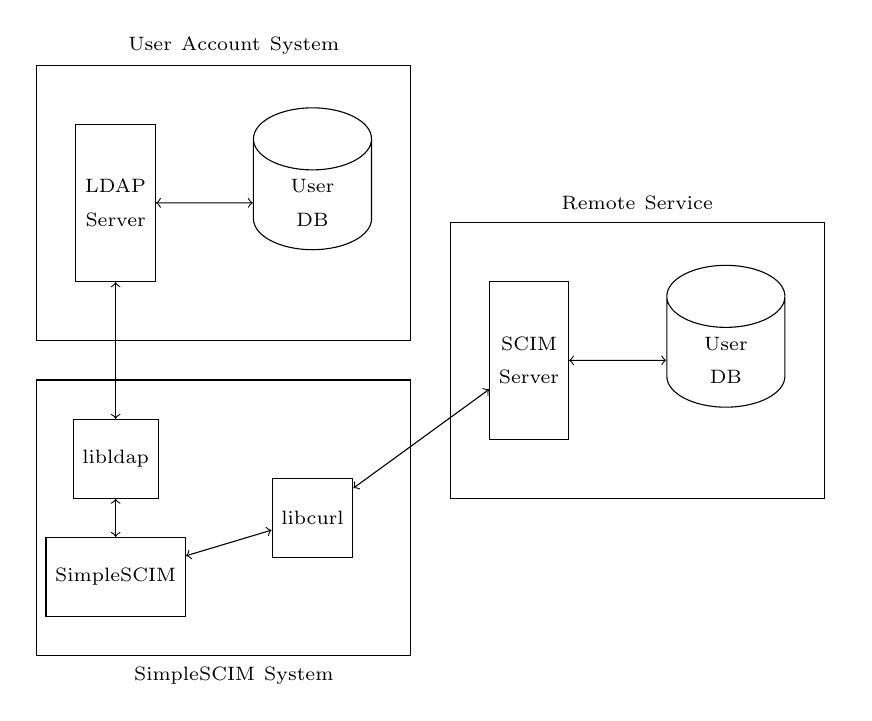
\begin{tikzpicture}
    % User Account System

    \node [text width=5cm, align=center] at (2.5,0.25)
          {\scriptsize User Account System};
    \draw (0,0) rectangle (4.75,-3.5);
    \node (ldapserver) [rectangle, draw, align=center,
                        minimum height=2cm]
          at (1,-1.75) {\scriptsize{LDAP} \\ \scriptsize{Server}};
    \node (userdb) [cylinder, shape border rotate=90, draw,
                    align=center, minimum width=1.5cm]
          at (3.5,-1.75) {\scriptsize{User} \\ \scriptsize{DB}};
    \draw[<->] (ldapserver) -- (userdb);

    % SimpleSCIM System

    \node [text width=5cm, align=center] at (2.5,-7.75)
          {\scriptsize SimpleSCIM System};
    \draw (0,-4) rectangle (4.75,-7.5);
    \node (libldap) [rectangle, draw, align=center,
                     minimum height=1cm]
          at (1,-5) {\scriptsize libldap};
    \node (simplescim) [rectangle, draw, align=center,
                        minimum height=1cm]
          at (1,-6.5) {\scriptsize SimpleSCIM};
    \node (libcurl) [rectangle, draw, align=center,
                     minimum height=1cm]
          at (3.5,-5.75) {\scriptsize libcurl};
    \draw[<->] (ldapserver) -- (libldap);
    \draw[<->] (libldap) -- (simplescim);
    \draw[<->] (simplescim) -- (libcurl);

    % Remote Service

    \node [text width=5cm, align=center] at (7.625,-1.75)
          {\scriptsize Remote Service};
    \draw (5.25,-2) rectangle (10,-5.5);
    \node (scimserver) [rectangle, draw, align=center,
                        minimum height=2cm]
          at (6.25,-3.75) {\scriptsize{SCIM} \\ \scriptsize{Server}};
    \node (userdbremote) [cylinder, shape border rotate=90, draw,
                          align=center, minimum width=1.5cm]
          at (8.75,-3.75) {\scriptsize{User} \\ \scriptsize{DB}};
    \draw[<->] (scimserver) -- (userdbremote);
    \draw[<->] (libcurl) -- (scimserver);
   \end{tikzpicture}
   \caption{Block diagram}
   \label{figure:block-diagram}
  \end{figure}

   \subsubsection{System interfaces}

   As illustrated in figure~\ref{figure:block-diagram}, SimpleSCIM
   interfaces different systems using different C libraries. The
   following system interfaces are used:

   \begin{enumerate}
    \item
     To perform local file operations when reading configuration
     files and when reading and writing cached files, the following
     wrappers on Linux system calls are used: \texttt{<unistd.h>},
     \texttt{<sys/types.h>}, \texttt{<sys/stat.h>} and
     \texttt{<fcntl.h>}.

    \item
     \texttt{<ldap.h>} by OpenLDAP is used to connect to a remote
     LDAP server and to receive user account data from that server
     according to specified filters.

    \item
     \texttt{<curl.h>} is used to send SCIM requests to the remote
     service.
   \end{enumerate}

   \newpage

   \subsubsection{User interfaces}

   SimpleSCIM is a command line program intended to be used on a
   UNIX like system. The user interface is two-fold; the execution
   of the program and the construction of the configuration files.
   To execute the program, a user using SimpleSCIM will type
   \texttt{SimpleSCIM file...} into a terminal. \texttt{file...} is a
   list of zero or more configuration files to be executed. Every
   configuration file specified in the list will be executed in given
   order, one at the time, to completion before moving on to the next
   configuration file. If there is a syntactical or semantic error
   in a configuration file, SimpleSCIM will print an error message to
   the terminal and move on to the next configuration file.

   A user of SimpleSCIM will also have to construct configuration
   files for every remote service in use. The format and contents of
   these configuration files are described in detail in
   appendix~\ref{appendix}.

   \subsubsection{Memory constraints}

   When SimpleSCIM parses a configuration file, the configuration
   file is read in its entirety into the system's primary memory.
   After a configuration file has been parsed, a hash table with the
   configuration file's variable/value-pairs is stored in the primary
   memory instead of the entire file.

   In order to remember the state of the previous execution of
   SimpleSCIM, the latest response from the LDAP server is stored on
   disk for every configuration file. If a configuration file
   specifies an LDAP filter that returns large amounts of user data,
   the cache files will be of equivalent large sizes.

  \subsection{Product functions}

  Using SimpleSCIM, the user will be able to create rules specifying
  the relationship between a subset of the local users and a remote
  service with a SCIM interface.

  SimpleSCIM uses cached results from previous executions to
  determine what needs to be done to the remote service's user
  account database. Given that the LDAP server is actively maintained
  and contains current and correct user account data, SimpleSCIM is
  well suited to run periodically using tools like \texttt{cron},
  to minimise active maintenance work.

  \subsection{User characteristics}

  There is mainly one type of user that uses SimpleSCIM; a system
  administrator in an institution or an entity with read access to
  an LDAP interface to the user account database, who is also
  responsible for giving users of the institute or entity access to
  a remote service.

  An example is the system administrator at a school with access to
  the student user account database. The school has an agreement with
  a study material platform and the teacher of one class wants their
  students to gain access to this study material platform. The
  teacher makes this request to the system administrator, who in turn
  creates a configuration file for the class and study material
  platform. Students might be enrolled late to the class, and
  students might drop out of the class during the semester, so the
  system administrator sets up a task in \texttt{cron} to execute
  this configuration file every day.

  \newpage

  \subsection{Constraints}

   \subsubsection{Regulatory policies}

   It is illegal to use SimpleSCIM to manage remote user accounts if
   the user's institution or entity does not have a
   ``personuppgiftsbiträdesavtal'' agreement with the remote service.

   \subsubsection{Parallel operation}

   Multiple processes running SimpleSCIM should not run the same
   configuration file concurrently, since this could corrupt the
   cache files.

   \subsubsection{Reliability requirements}

   SimpleSCIM's reliability depends on the uptime of the system it
   runs in and the stability of the internet connection to the LDAP
   server and the SCIM server.

   \subsubsection{Criticality of the application}

   SimpleSCIM could potentially enter a corrupted state if the cache
   files are corrupted or deleted. SimpleSCIM cannot know for example
   if a user has been deleted and should be removed from the remote
   service if the cache files are corrupted.

   \subsubsection{Safety and security considerations}

   SimpleSCIM will establish secure connections to both the LDAP
   server and the SCIM server according to each protocol's
   recommendation.

  \subsection{Assumptions and dependencies}

  This document makes the following assumptions on the system used
  for executing SimpleSCIM:

  \begin{enumerate}
   \item
    The operating system uses a Linux kernel.

   \item
    The user account data is accessible through an LDAP server.

   \item
    A remote service has a SCIM interface to its user account
    database.
  \end{enumerate}

  \noindent
  The following dependencies are also present:

  \begin{enumerate}
   \item
    The LDAP protocol is used and accessed using \texttt{libldap} by
    OpenLDAP.

   \item
    The SCIM protocol is used and accessed using \texttt{libcurl}.

   \item
    Both the LDAP server and the SCIM server are accessed over the
    internet. Both servers must therefore be addressable over IP or
    IPv6.
  \end{enumerate}

 \newpage

 \section{Specific requirements}
 \label{section:specific-requirements}

 This section contains all functional and quality requirements of the
 software. It gives a detailed description of the system and all its
 features.

  \subsection{External interfaces}

  The software's inputs and outputs can be specified on different
  layers. The first layer is the terminal input and output. A user
  specifies which configuration files to execute as command line
  arguments to the software. The terminal output is quiet if
  everything was successful, otherwise an error message is printed.

  The second layer is the configuration file's contents and error
  messages related to it's syntactical and semantic correctness. The
  configuration file is the user input, since the configuration files
  are created manually. The exact syntax and semantics of the
  configuration files are described in detail in
  appendix~\ref{appendix}.

  The third layer is the LDAP transaction. The filter is specified
  in the configuration file as well as authentication information,
  and any output depends on whether LDAP accepts the provided input
  or an error occurs.

  The fourth layer is the SCIM transaction. The input is JSON objects
  specified in the configuration file including the relation from
  LDAP attribute to JSON field. The output is dependent on whether
  the remote server accepts the SCIM request or not. Should an error
  occur, the error message will be printed to the terminal.

  Error messages can also be redirected to a log file using UNIX
  commands if that is more convenient for the user.

  \subsection{Feature}

  The following features are required:

  \begin{enumerate}
   \item
    The software can fetch user account data from an existing LDAP
    server according to specified selection filters.

   \item
    The software can fetch user groups from an LDAP server according
    to specified selection filters.

   \item
    The software can convert the user account data and group
    information received from the LDAP server into a specified SCIM
    format according to the rules in the configuration file.

   \item
    The software can connect to both the LDAP server and the SCIM
    server securely with the settings specified in the configuration
    file.

   \item
    The software can transmit user account information to the remote
    system using SCIM so that user accounts remotely can be created,
    modified and removed from the remote service when equivalent
    operation is executed in the LDAP server that is the source of
    the user account data.
  \end{enumerate}

 \newpage

 \appendix

 \section{Code}
 \label{appendix}

 The code for SimpleSCIM is hosted on GitHub on the following link:

 \begin{center}
  \url{https://github.com/MaxWallstedt/SimpleSCIM}
 \end{center}

 \noindent
 This link also contains detailed compilation instructions, detailed
 technical specification for the configuration files and copyright
 information for the software.

\end{document}
